% Copyright 2026 Sreeram Anil
% SPDX-License-Identifier: CC-BY-4.0
% =============================================================================
%  Quaternion complementary filter — attitude (AHRS) family
% =============================================================================
\chapter{Quaternion Complementary Filter (Complementary)}
\label{ch:att-complementary}

\section*{At a glance}
\begin{tabular}{@{}l>{\raggedright\arraybackslash}p{0.76\textwidth}@{}}
Family & attitude / AHRS \\
Header & \texttt{include/estkit/attitude/complementary.hpp} \\
Registered name & \texttt{Complementary} \\
State & unit quaternion $\bm{q}\in S^3$ (4 reals); no bias state, no covariance \\
Cost per step & $\approx300$ flops, six transcendental calls;
  $0.26$--$\SI{0.33}{\micro\second}$/step, 272\,bytes \\
Primary references & \cite{higgins1975complementary,euston2008,titterton2004,markleycrassidis2014} \\
\end{tabular}

\section{Motivation and aerospace relevance}
Every attitude-and-heading reference system solves the same signal-processing problem twice over:
a triad of rate gyroscopes gives an attitude \emph{increment} that is accurate over a second and
useless over an hour, while a triad of accelerometers and magnetometers gives an attitude
\emph{absolute} measurement that is noisy and disturbance-prone over a second and drift-free over
an hour. The two error spectra are complementary: gyro error grows like $\sqrt{t}$ (angle random
walk) plus $t$ (bias), whereas the vector-observation error is broadband but stationary. A filter
that high-passes the gyro and low-passes the vector solution, with the two transfer functions
summing to unity, removes both errors without ever computing a covariance.

Higgins~\cite{higgins1975complementary} made the connection precise: for a two-state model
(signal plus integrated bias) the steady-state Kalman filter \emph{is} a complementary filter, and
the single cross-over frequency of the complementary pair is the only degree of freedom the Kalman
filter has once the noise ratio is fixed. That is why a filter with one knob per channel can be
competitive with a six-state Kalman filter when the noise statistics are stationary --- and why it
cannot be when they are not.

The specific failure that motivates the second half of this chapter is a fixed-wing one. In a
\emph{coordinated} turn the pilot (or autopilot) holds the lateral specific force at zero, so the
accelerometer points along the body $z$ axis and reports \emph{zero bank angle} no matter how steep
the turn. The magnitude of the specific force changes only as $1/\cos\phi$ ($+10\,\%$ at
$\phi=25^\circ$), so a magnitude check cannot detect the condition either. Euston, Coote, Mahony,
Kim and Hamel~\cite{euston2008} proposed the standard fix for small UAVs: use the airspeed and the
turn rate to reconstruct the centripetal term and subtract it from the accelerometer before the
tilt is extracted. This chapter implements that correction as an option and measures exactly what
it is worth --- and what it costs. (The alternative, when a GNSS velocity is available, is to
reconstruct $\dot{\bm{v}}_b$ outright; see Hua~\cite{hua2010}.)

\section{Problem statement and assumptions}
Let $\bm{q}$ be the unit quaternion mapping the BODY frame (FRD) to the NAVIGATION frame (NED),
with rotation matrix $\bm{R}(\bm{q})$, so that $\bm{v}_{\text{nav}}=\bm{R}\bm{v}_{\text{body}}$.
Throughout this family $\bm{R}$ denotes a rotation and measurement covariances are written
$\bm{\Sigma}$, to avoid a clash with the usual $\mR$; the quaternion conventions are those of
Kuipers~\cite{kuipers1999} and the reference field is an IGRF~\cite{thebault2015igrf} value for
central Europe.

The sensors, at $\dt=\SI{10}{\milli\second}$, are
\begin{align}
\bm{\omega}_y &= \bm{\omega} + \bm{b} + \bm{n}_v, &&\bm{b} \text{ a slowly varying gyro bias},\label{eq:cf-gyro}\\
\bm{f} &= \bm{R}^\T(\bm{a}_{\text{nav}} - \bm{g}_{\text{nav}}) + \bm{b}_a + \bm{n}_a, &&\bm{g}_{\text{nav}} = [0,0,g]^\T,\label{eq:cf-acc}\\
\bm{m} &= \bm{R}^\T\bm{m}_{\text{nav}} + \bm{b}_m + \bm{n}_m, &&\bm{m}_{\text{nav}} = B[\cos I,0,\sin I]^\T,\label{eq:cf-mag}
\end{align}
with $B=\SI{48}{\micro\tesla}$ and magnetic inclination $I=65^\circ$. Note the sign convention in
\eqref{eq:cf-acc}: at rest $\bm{f}=\bm{R}^\T[0,0,-g]^\T$, so the NAV reference of the
\emph{normalised} accelerometer is $\bm{d}_a=[0,0,-1]^\T$ (``up'' in NED).

The filter assumes (i) $\bm{a}_{\text{nav}}\approx\bm{0}$ on average, so that $\bm{f}$ measures
$-\bm{R}^\T\bm{g}_{\text{nav}}$ at low frequency, (ii) $\bm{m}_{\text{nav}}$ is known, and
(iii) $\bm{b}$ is small enough that $\norm{\bm{b}}\tau$ is an acceptable steady-state error, because
\emph{the filter has no bias state}. It estimates $\bm{q}$ only.

\section{Derivation}

\subsection{The complementary pair}
Write $\theta$ for any one attitude channel, $\theta_g$ for the gyro-integrated estimate and
$\theta_v$ for the vector-observation estimate. With the first-order low-pass
$G(s)=1/(\tau s+1)$,
\begin{equation}
\hat\theta(s) = \big(1-G(s)\big)\,\theta_g(s) + G(s)\,\theta_v(s),
\qquad \big(1-G\big)+G \equiv 1,
\label{eq:cf-pair}
\end{equation}
so a common component passes unchanged whatever $\tau$ is: the filter is unbiased by construction.
Substituting the error models $\theta_g=\theta+\varepsilon_g$, $\theta_v=\theta+\varepsilon_v$
gives $\hat\theta-\theta = (1-G)\varepsilon_g + G\varepsilon_v$: the gyro error is high-passed
(so its drift is removed, at the price of leaving $\tau\dot\varepsilon_g$) and the vector error is
low-passed (so its noise is attenuated by $\sqrt{\dt/2\tau}$). For a constant gyro bias $b$ the
residual is exactly
\begin{equation}
\lim_{t\to\infty}\big(\hat\theta-\theta\big) = b\,\tau ,
\label{eq:cf-bias}
\end{equation}
which is the single most important design equation of the whole method: $\tau=\SI{1}{\second}$ and
$b=\SI{0.5}{\degree\per\second}$ cost $0.5^\circ$; the same $\tau$ with
$b=\SI{3}{\degree\per\second}$ costs $3^\circ$.

\subsection{Quaternion implementation}
Equation~\eqref{eq:cf-pair} is scalar; attitudes do not add. The implementation therefore performs
the blend \emph{multiplicatively}, which keeps $\norm{\bm{q}}=1$ exactly and is valid for
arbitrarily large corrections.

\paragraph{1. Gyro branch (high-pass).} Exact exponential propagation of
$\dot{\bm{q}}=\tfrac12\bm{q}\otimes[0,\bm{\omega}_y]$ over one sample,
\begin{equation}
\bm{q}^- = \bm{q}\otimes\exp\!\big(\bm{\omega}_y\dt\big),\qquad
\exp(\bm{\rho}) = \Big[\cos\tfrac{\norm{\bm{\rho}}}{2},\;
 \tfrac{\bm{\rho}}{\norm{\bm{\rho}}}\sin\tfrac{\norm{\bm{\rho}}}{2}\Big].
\label{eq:cf-prop}
\end{equation}

\paragraph{2. Tilt branch (low-pass).} From the corrected specific force $\bm{a}_c$ (below),
$\bm{d}_b = -\bm{a}_c/\norm{\bm{a}_c}$ is the body-frame ``down'' direction, i.e. the third row of
$\bm{R}$, $\bm{d}_b = [-\sin\theta,\;\cos\theta\sin\phi,\;\cos\theta\cos\phi]^\T$, hence
\begin{equation}
\theta_a = \arcsin\!\big(-d_{b,1}\big),\qquad \phi_a = \operatorname{atan2}(d_{b,2},d_{b,3}),
\label{eq:cf-tilt}
\end{equation}
with the $\arcsin$ argument clamped to $[-1,1]$. A measurement quaternion is assembled from the
\emph{accelerometer} roll and pitch and the \emph{current} heading, so that the tilt branch cannot
move the heading:
\begin{equation}
\bm{q}_{\text{meas}} = \bm{q}_{ZYX}(\phi_a,\theta_a,\hat\psi),\qquad
\bm{\delta} = \log\!\big(\bm{q}^{-*}\otimes\bm{q}_{\text{meas}}\big)\in\real^3,
\label{eq:cf-delta}
\end{equation}
and a fraction of the body-frame rotation vector $\bm{\delta}$ is applied,
\begin{equation}
\bm{q}^+ = \bm{q}^-\otimes\exp\!\big(\gamma_a\,\bm{\delta}\big),\qquad
\gamma_a = w_a\,\frac{\dt}{\tau_a+\dt},
\label{eq:cf-tiltblend}
\end{equation}
which is the exact discretisation of \eqref{eq:cf-pair} with $G(s)=1/(\tau_a s+1)$ lifted to
$SO(3)$ along the geodesic joining $\bm{q}^-$ to $\bm{q}_{\text{meas}}$.

\paragraph{3. Heading branch (low-pass).} With the current roll and pitch, the level-frame field is
$\bm{m}_{\text{lev}}=\bm{R}_y(\hat\theta)\bm{R}_x(\hat\phi)\bm{m}=\bm{R}_z(\psi)^\T\bm{m}_{\text{nav}}$,
so with $x_h,y_h$ its first two components and $D=\operatorname{atan2}(m_{\text{nav},2},m_{\text{nav},1})$
the declination,
\begin{equation}
x_h = m_1 c_\theta + m_2 s_\theta s_\phi + m_3 s_\theta c_\phi,\quad
y_h = m_2 c_\phi - m_3 s_\phi,\quad
\psi_m = \operatorname{atan2}(-y_h,x_h) + D .
\label{eq:cf-head}
\end{equation}
The heading error $e_\psi = \operatorname{wrap}(\psi_m-\hat\psi)$ is corrected by a rotation about
the \emph{navigation} vertical, i.e. by pre-multiplication, which by construction leaves roll and
pitch untouched:
\begin{equation}
\bm{q}^{++} = \big[\cos\tfrac{u}{2},0,0,\sin\tfrac{u}{2}\big]\otimes\bm{q}^+ ,\qquad
u = w_m\,\frac{\dt}{\tau_m+\dt}\,e_\psi .
\label{eq:cf-headblend}
\end{equation}

\subsection{The specific-force disturbance and the centripetal correction}
Differentiating $\bm{v}_{\text{nav}}=\bm{R}\bm{v}_b$ and substituting into \eqref{eq:cf-acc},
\begin{equation}
\bm{f} = \dot{\bm{v}}_b + \bm{\omega}\times\bm{v}_b - \bm{R}^\T\bm{g}_{\text{nav}} .
\label{eq:cf-sf}
\end{equation}
For an aircraft flying along its $x$ axis at true airspeed $V$ with $\dot V\approx0$ we have
$\bm{v}_b\approx[V,0,0]^\T$ and therefore the Euston et al.~\cite{euston2008} correction
\begin{equation}
\bm{a}_c \;=\; \bm{f} - \bm{\omega}_y\times[V,0,0]^\T
 \;=\; \big[f_1,\; f_2-\omega_{y,3}V,\; f_3+\omega_{y,2}V\big]^\T
 \;\approx\; -\bm{R}^\T\bm{g}_{\text{nav}} .
\label{eq:cf-centri}
\end{equation}
Two consequences follow immediately and are both visible in the benchmark.
\begin{remark}[What the correction buys]
In a coordinated turn at bank $\phi$ and turn rate $\dot\psi$ the lateral specific force is
$f_2 \approx \dot\psi V\cos\phi - g\sin\phi \approx 0$, so the uncorrected tilt
\eqref{eq:cf-tilt} returns $\phi_a\approx0$: an error of the \emph{full} bank angle,
$23^\circ$ on this mission, held for the entire $\SI{60}{\second}$ of each turn.
\end{remark}
\begin{remark}[What it costs]\label{rem:cf-cost}
$\bm{\omega}_y$ in \eqref{eq:cf-centri} is the \emph{raw} rate, bias included, because this filter
has no bias state. A rate error $\delta\omega$ produces a specific-force error $V\delta\omega$ and
hence a tilt error
\begin{equation}
\delta\phi \;\approx\; \frac{V}{g}\,\delta\omega ,
\label{eq:cf-amplify}
\end{equation}
an amplification of $V/g = 45/9.81 = 4.6$ seconds. A $\SI{1}{\degree\per\second}$ bias, harmless in
\eqref{eq:cf-bias} with $\tau=\SI{1}{\second}$, becomes a $4.6^\circ$ tilt error through
\eqref{eq:cf-centri}. The correction therefore requires a calibrated gyro, and the benchmark's
\texttt{gyro\_bias} scenario is designed to expose exactly this.
\end{remark}

\subsection{Disturbance de-rating}
Both branches are gated by a weight built from the low-pass-filtered magnitude anomaly of the
observation. With $\bar{y}$ the filtered magnitude, $y_{\text{ref}}$ its nominal value, a dead-zone
$d$ and a slope $k$,
\begin{equation}
\sigma_x = k\,\max\big(0,\;\abs{\bar{y}-y_{\text{ref}}}-d\big),\qquad
w = \frac{\sigma_0^2}{\sigma_0^2+\sigma_x^2},\qquad
\sigma_0^2=\sigma_{\text{sensor}}^2+\sigma_{\text{extra}}^2,
\label{eq:cf-weight}
\end{equation}
and $w\!:=\!0$ if $\sigma_x$ exceeds a rejection threshold. Expression \eqref{eq:cf-weight} is the
scalar Kalman gain ratio: it is the fixed-gain filter's substitute for an adaptive $\bm{\Sigma}$.
The magnitude is low-passed \emph{before} the comparison so that zero-mean vibration, which inflates
$\E{\norm{\bm{f}}}$ only by $\sqrt{g^2+3\sigma^2}-g=\SI{0.16}{\metre\per\second\squared}$ at
$\sigma=\SI{1.05}{\metre\per\second\squared}$, does not trip the gate.

\section{Algorithm}
\begin{algorithm}[H]
\caption{Complementary --- one sampling period ($\dt=\SI{10}{\milli\second}$)}
\begin{algorithmic}[1]
\Require $\bm{q}_{k-1}$, $\bm{\omega}_y$, $\bm{f}$, $\bm{m}$; $\tau_a,\tau_m,V$
\State $\bm{q}\gets\bm{q}_{k-1}\otimes\exp(\bm{\omega}_y\dt)$, normalise \Comment{high-pass branch, \eqref{eq:cf-prop}}
\State $\bm{a}_c\gets\bm{f}-\bm{\omega}_y\times[V,0,0]^\T$ \Comment{centripetal correction, \eqref{eq:cf-centri}}
\State $w_a\gets$ \eqref{eq:cf-weight} from $\norm{\bm{a}_c}$ versus $g$
\If{$w_a>0$}
  \State $(\phi_a,\theta_a)\gets$ \eqref{eq:cf-tilt}; \; $\hat\psi\gets$ yaw of $\bm{q}$
  \State $\bm{\delta}\gets\log(\bm{q}^*\otimes\bm{q}_{ZYX}(\phi_a,\theta_a,\hat\psi))$; \;
         $\bm{q}\gets\bm{q}\otimes\exp\!\big(w_a\tfrac{\dt}{\tau_a+\dt}\bm{\delta}\big)$, normalise
\EndIf
\State $w_m\gets$ \eqref{eq:cf-weight} from $\norm{\bm{m}}$ versus $\norm{\bm{m}_{\text{nav}}}$
\If{$w_m>0$}
  \State $(\hat\phi,\hat\theta,\hat\psi)\gets$ Euler of $\bm{q}$; \; $\psi_m\gets$ \eqref{eq:cf-head}
  \State $u\gets w_m\tfrac{\dt}{\tau_m+\dt}\operatorname{wrap}(\psi_m-\hat\psi)$;\;
         $\bm{q}\gets[\cos\frac{u}{2},0,0,\sin\frac{u}{2}]\otimes\bm{q}$, normalise
\EndIf
\Ensure $\bm{q}_k$
\end{algorithmic}
\end{algorithm}

\section{Application to the benchmark flight}
The registered configuration is $\tau_a=\SI{1}{\second}$, $\tau_m=\SI{2}{\second}$ (the classical
$1$--$\SI{2}{\second}$ band), centripetal correction \emph{on} with the nominal cruise airspeed
$V=\SI{45}{\metre\per\second}$, and gating on with
$\sigma_{a,\text{extra}}=\SI{1}{\metre\per\second\squared}$, $d_a=\SI{2}{\metre\per\second\squared}$,
$k_a=5$, $\sigma_{m,\text{extra}}=\SI{1.5}{\micro\tesla}$, $d_m=\SI{2}{\micro\tesla}$, $k_m=10$.

The accelerometer dead-zone is deliberately wide ($\SI{2}{\metre\per\second\squared}$): after the
correction \eqref{eq:cf-centri} the residual magnitude error is of order $V\norm{\delta\bm{\omega}}$
(Remark~\ref{rem:cf-cost}), so a tight gate would switch the tilt branch \emph{off} exactly when a
gyro bias is present, leaving pure open-loop integration. That failure mode was observed during
tuning: with $d_a=\SI{0.3}{\metre\per\second\squared}$ and $k_a=15$ the \texttt{gyro\_bias} RMS ran
past $100^\circ$ instead of the $\SI{17.6}{\degree}$ of the registered configuration.

\section{Implementation notes}
The state is one quaternion; \code{sizeof} is 272\,bytes, essentially all of it \code{Options} and
the two gate low-pass filters (the estimate itself is $4\times8$\,bytes). There is no matrix algebra
at all, but the filter is nevertheless the \emph{slowest} of the light filters at
$0.26$--$\SI{0.33}{\micro\second}$/step against Madgwick's $0.09$: the cost is six transcendental
calls per step (\code{to\_euler} twice, \code{from\_euler}, \code{log}, two \code{exp}). A
production implementation that works entirely with cross products, like the Mahony filter of
Chapter~\ref{ch:att-mahony}, removes all of them.

Numerical hygiene: the quaternion is renormalised after each of the three multiplications; the
$\arcsin$ argument in \eqref{eq:cf-tilt} is clamped; both branches are skipped if the corresponding
measurement magnitude is below $10^{-3}$; $\exp$ falls back to the first-order form below
$10^{-9}$\,rad. The heading error is wrapped to $(-\pi,\pi]$ before the blend, so a
$\pm180^\circ$ crossing costs nothing. There is no covariance and hence no positive-definiteness to
maintain. The single-precision build reproduces the double-precision RMS to three digits
(the single-seed \texttt{nominal} RMS agrees to four digits).

Limitations, all structural: no bias state (\eqref{eq:cf-bias}), no covariance so no way to weight
roll against yaw, and an airspeed-dependent correction that a gyro bias corrupts by $V/g$.

\section{Benchmark results}
% Copyright 2026 Sreeram Anil
% SPDX-License-Identifier: CC-BY-4.0
\begin{table}[H]\centering\footnotesize\setlength{\tabcolsep}{3.5pt}\caption{Complementary: attitude benchmark (mean over seeds; all angles in degrees; $t_\mathrm{conv}$: first time the attitude error stays below 2$^\circ$ for 30\,s; bias RMSE in deg/s; 272 bytes of state).}\label{tab:imu_Complementary}
\begin{tabular}{lrrrrrrrrcr}\toprule scenario & RMS & roll & pitch & yaw & max & RMS$_\mathrm{ss}$ & $t_\mathrm{conv}$ [s] & bias RMSE & lost & ns/step \\ \midrule
nominal & 6.57 & 2.78 & 1.18 & 5.80 & 17.5 & 7.91 & 37 & 1.03 & no & 362 \\
init\_error & 6.79 & 2.88 & 1.37 & 5.98 & 46.3 & 7.91 & 37 & 1.03 & no & 363 \\
gyro\_bias & 17.58 & 7.41 & 2.20 & 15.89 & 28.5 & 17.44 & -- & 3.80 & no & 373 \\
mag\_disturbance & 6.71 & 2.78 & 1.18 & 5.97 & 20.1 & 7.91 & 37 & 1.03 & no & 357 \\
vibration & 6.58 & 2.79 & 1.24 & 5.79 & 17.5 & 7.94 & 37 & 1.03 & no & 384 \\
high\_dynamics & 6.58 & 2.79 & 1.18 & 5.81 & 17.4 & 7.91 & 37 & 1.03 & no & 364 \\
\bottomrule\end{tabular}\end{table}

\begin{figure}[H]\centering
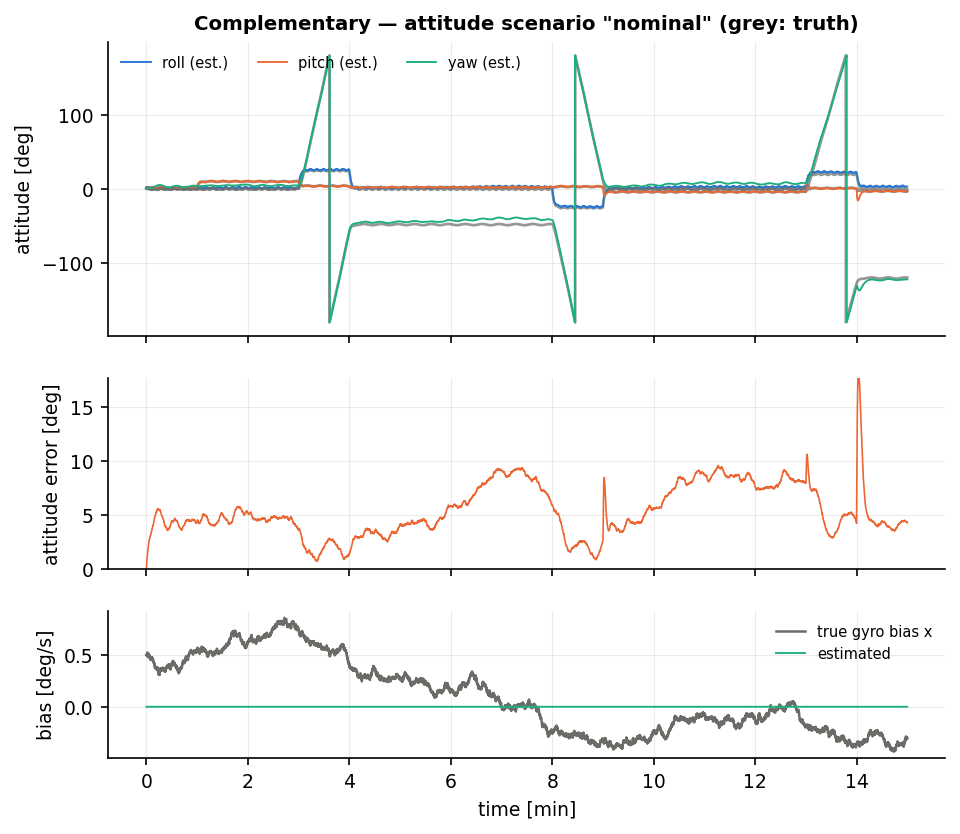
\includegraphics[width=\textwidth]{figures/imu_Complementary_nominal.png}
\caption{Complementary filter on the nominal mission: true and estimated Euler angles (top), total
angular error (middle), gyro-bias channel (bottom).}
\end{figure}
\begin{figure}[H]\centering
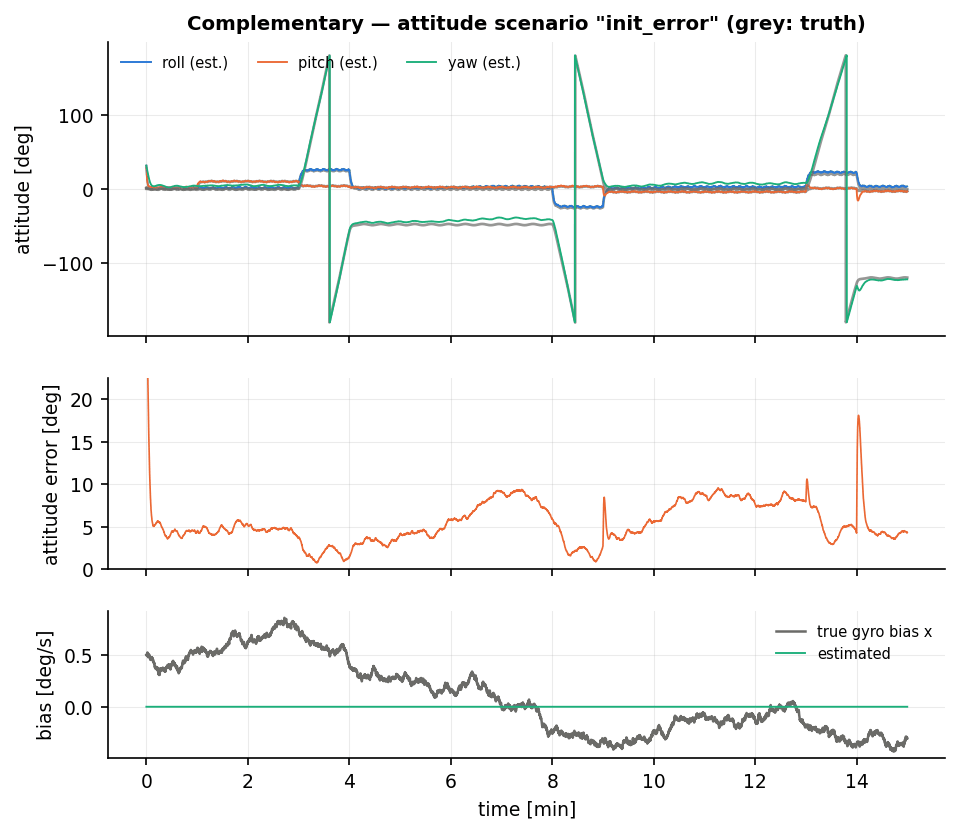
\includegraphics[width=\textwidth]{figures/imu_Complementary_init_error.png}
\caption{Complementary filter with a $30^\circ$ initial error on each Euler axis ($46.6^\circ$ of
total attitude error).}
\end{figure}
\begin{figure}[H]\centering
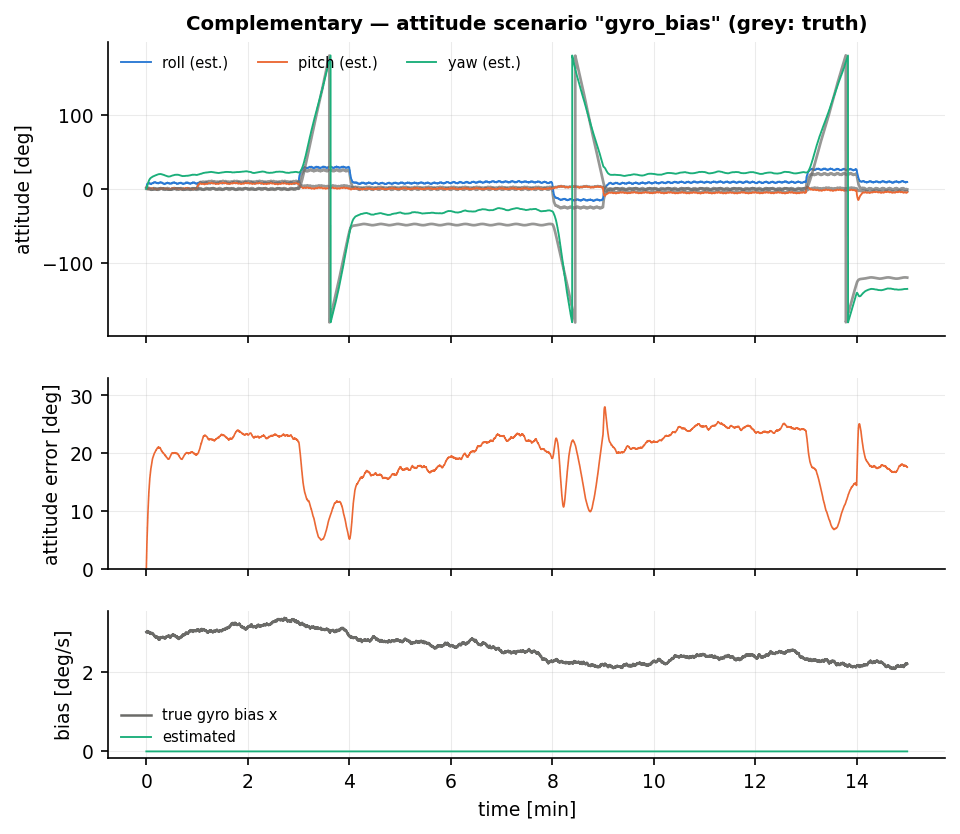
\includegraphics[width=\textwidth]{figures/imu_Complementary_gyro_bias.png}
\caption{Complementary filter on \texttt{gyro\_bias} ($\SI{3}{\degree\per\second}$ per axis): with
no bias state the centripetal correction \eqref{eq:cf-centri} multiplies the rate error by
$V/g\approx4.6$, and the tilt error it produces is amplified again into heading by the
$65^\circ$ magnetic dip.}
\end{figure}

On \texttt{nominal} the filter reaches $\text{RMS}=\SI{6.57}{\degree}$ (roll $2.78$, pitch $1.18$,
yaw $\SI{5.80}{\degree}$), $\text{RMS}_{\text{ss}}=\SI{7.91}{\degree}$, peak $\SI{17.5}{\degree}$, at
$\SI{362}{\nano\second}$/step and 272\,bytes. It passes the convergence test at
$t=\SI{37}{\second}$ --- the reduction of the dataset's residual hard iron to
$\SI{0.42}{\micro\tesla}$ brought its error briefly below $2^\circ$ --- and it is never marked
lost, on any scenario. Its \emph{bias} RMSE column simply reproduces the true bias magnitude
($1.03$ and $\SI{3.80}{\degree\per\second}$), because the filter has no bias state and reports zero.

Numbers quoted from the table are three-seed means; the ablations below are single-seed (seed~1)
diagnostics and are internally consistent with each other, not with the table to the last digit.

\paragraph{The centripetal correction is worth a factor of three.} Measured on \texttt{nominal}
with $\tau_a=\SI{1}{\second}$: $V=0$ (no correction) gives $\SI{18.36}{\degree}$, $V=20$ gives
$9.92$, $V=30$ gives $6.87$, $V=45$ (registered, the true cruise airspeed) gives $5.89$, and
$V=60$ gives $\SI{9.56}{\degree}$. The optimum sits at the true airspeed and the penalty for a
$\pm33\,\%$ airspeed error is $3$--$\SI{4}{\degree}$: the correction is useful but not forgiving.
Per flight phase (registered configuration, seed~1) the error is
\[
4.26\;/\;4.71\;/\;2.01\;/\;6.24\;/\;3.34\;/\;7.40\;/\;6.91\;/\;5.02\ \SI{}{\degree}
\]
for take-off / climb / turn\,1 / cruise / turn\,2 / descent / turn\,3 / final: \emph{with} the
correction the turns are among the \emph{best} phases, not the worst. Without it the turn phases are
$40$--$\SI{45}{\degree}$, exactly like the memory-less estimators of Chapters~\ref{ch:att-triad}
and~\ref{ch:att-quest}.

\paragraph{The gyro bias is the price.} On \texttt{gyro\_bias} ($\SI{3}{\degree\per\second}$ per
axis) the RMS rises to $\SI{17.58}{\degree}$, while the same filter with $V=0$ gives
$\SI{19.22}{\degree}$ --- i.e. the correction has almost stopped helping.
Equation~\eqref{eq:cf-amplify} predicts the size: the $y$ and $z$ bias components of $1.8$ and
$\SI{1.2}{\degree\per\second}$ give $V\delta\omega=1.41$ and
$\SI{0.94}{\metre\per\second\squared}$, i.e. $8.2^\circ$ and $5.5^\circ$ of tilt error, and the
measured roll RMS is $\SI{7.41}{\degree}$. The magnetic-dip amplification discussed below then
turns that into $\SI{15.89}{\degree}$ of heading error. This is the cleanest demonstration in the
family of why the bias must be a state: the six-state filters of Chapters~\ref{ch:att-mekf}
and~\ref{ch:att-iekf} are unaffected by this scenario ($\SI{2.48}{\degree}$, unchanged from
nominal).

\paragraph{Tuning sensitivity.} With the correction on, $\tau_a=0.5/1/\SI{2}{\second}$ give
$5.59/5.89/\SI{6.68}{\degree}$ on \texttt{nominal} and $16.4/20.1/\SI{27.8}{\degree}$ on
\texttt{gyro\_bias}, the latter following \eqref{eq:cf-bias} almost exactly. Without the correction
the ordering reverses on \texttt{nominal} ($19.0/18.4/16.9$), because a slower filter rejects more
of the manoeuvre disturbance. $\SI{1}{\second}$ is the compromise, and it is inside the range the
assignment prescribes.

\paragraph{Disturbance scenarios.} \texttt{mag\_disturbance} (a $\SI{25}{\micro\tesla}$ offset for
$\SI{20}{\second}$ at $t=\SI{300}{\second}$) costs $\SI{0.14}{\degree}$ of mission RMS
($6.71$ against $6.57$), because the magnitude gate sees $\norm{\bm{m}}$ rise from $48$ to
$\SI{54}{\micro\tesla}$ and switches the heading branch off; with the gate disabled the same
scenario costs $\SI{3.2}{\degree}$ ($9.12$ against $\SI{5.87}{\degree}$, seed~1).
\texttt{vibration} ($\sigma_a=\SI{1.05}{\metre\per\second\squared}$) is free ($6.58$): the
$\SI{1}{\second}$ low-pass attenuates broadband accelerometer noise by
$\sqrt{\dt/2\tau_a}=0.07$. \texttt{high\_dynamics} is free as well ($6.58$).
\texttt{init\_error} costs $\SI{0.2}{\degree}$ of mission RMS but takes $\SI{17.9}{\second}$ to
bring a $46.6^\circ$ error below $5^\circ$ --- the price of a fixed first-order low-pass whose tilt
and heading loops have to unwind sequentially.

\paragraph{Where the residual $\SI{5.8}{\degree}$ of yaw comes from.} After the recalibration of the
simulated compass this is now \emph{almost entirely} dip-amplified tilt error, and the hard iron is
a minor term. The dataset's residual hard-iron offset is
$\bm{b}_m=[0.30,-0.15,0.25]^\T\,\SI{}{\micro\tesla}$, $\norm{\bm{b}_m}=\SI{0.42}{\micro\tesla}$ or
$0.87\,\%$ of the field; fed to an \emph{exact} tilt-compensated compass it alone produces only
$\SI{0.65}{\degree}$ RMS ($\SI{1.12}{\degree}$ peak) of heading error. The dominant term is the
leakage of tilt error into the tilt-compensated heading with gain $\tan I = 2.14$ at $I=65^\circ$:
the residual roll RMS of $\SI{2.78}{\degree}$ --- itself the $V/g$-amplified gyro-bias random walk
of \eqref{eq:cf-amplify} --- contributes $2.78\times2.14\approx\SI{5.9}{\degree}$, which together
with $\SI{0.65}{\degree}$ of hard iron accounts for the measured $\SI{5.80}{\degree}$. Reducing the
tilt error, not the magnetometer error, is what would improve this filter.

\section{Summary}
Use the complementary filter when the platform is calibrated, the noise statistics are stationary
and the code budget is a few hundred bytes: it costs one quaternion, has one knob per channel, and
its steady-state error is the closed-form $b\tau$ of \eqref{eq:cf-bias}. On a fixed-wing aircraft
it is unusable without the Euston centripetal correction --- $18.4^\circ$ versus $\SI{6.6}{\degree}$
RMS here --- and the correction in turn amplifies gyro-bias error by $V/g\approx4.6$, which is why
this filter is $\SI{17.6}{\degree}$ on \texttt{gyro\_bias} where the six-state filters of
Chapters~\ref{ch:att-mekf} and \ref{ch:att-iekf} are $\SI{2.5}{\degree}$. Do not use it when the
gyro bias is unknown, when the disturbance statistics change during the mission, or when a
covariance is needed downstream.
